\section{Linear Approximation}
\label{sec:linear-approximation}

To test the schedulability of a task $\tau_k$,
Corollary~\ref{corollary:general-framework} implies to test all the
possible vector assignments $\vec{x} = (x_1, x_2, \ldots, x_{k-1})$ to get the tightest result (under our analysis). Therefore, $2^{k-1}$ possible combinations should be tested, implying exponential time complexity. In this section, we thus provide a solution to reduce the time complexity associated to
Corollary~\ref{corollary:general-framework}. Indeed, using a linear approximation of the test in Eq.~(\ref{eq:TDA-suspension-tighter}), a good vector assignment can be derived in linear time. 

By the definition of the ceiling operator, it holds that:
{\footnotesize \begin{align}
&C_k + S_k + \sum_{i=1}^{k-1}\ceiling{\frac{t+\sum_{\ell=i}^{k-1}x_\ell S_\ell+(1-x_i)(R_i-C_i)}{T_i}} C_i \nonumber\\
\leq& C_k + S_k  +   \sum_{i=1}^{k-1} \left(\frac{t+\sum_{\ell=i}^{k-1}x_\ell S_\ell +(1-x_i)(R_i-C_i)}{T_i} +1\right) C_i \nonumber\\
=& C_k + S_k  + \sum_{i=1}^{k-1} \left(U_i\cdot t + C_i+U_i (1-x_i)(R_i-C_i) + U_i\sum_{\ell=i}^{k-1}x_\ell S_\ell \right) \label{eq:linear_step1}
\end{align}}




\begin{figure*}[t!]
  \centering
  \subfloat[Varying the number of tasks $n$, $U'=0.95$, $r_{\min} = 0.05$, $r_{\max} = 0.5$]{\label{fig:plot1} 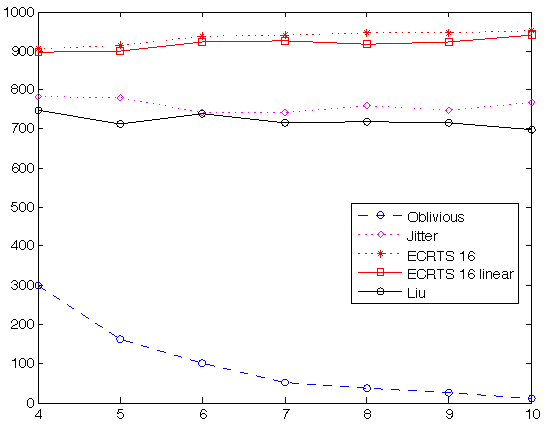
\includegraphics[width=0.253\textwidth]{../figures/experiments/varyingn_smin=5_smax=50_U=0_95_T=100-10000_1000runs_croped.pdf}}
  \subfloat[Varying $r_{\max}$ (unit: \%), $U'=1$, $n=8$, $r_{\min} = 0.05$]{\label{fig:plot2} 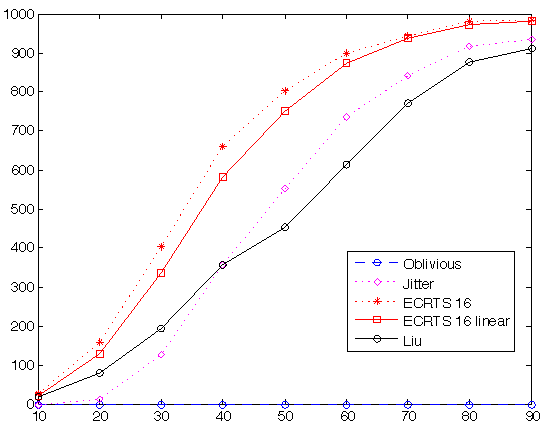
\includegraphics[width=0.23\textwidth]{../figures/experiments/varyingSmax_smin=5_U=1_n=8_T=100-10000_1000runs_croped.pdf}}
  \subfloat[Varying $U'$, $n=8$, $r_{\min} = 0.05$, $r_{\max} = 0.5$]{\label{fig:plot3} 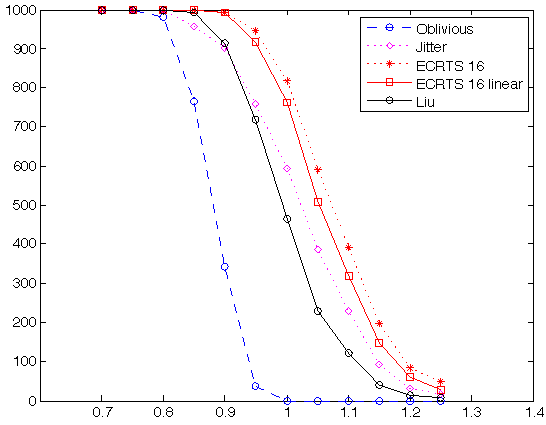
\includegraphics[width=0.23\textwidth]{../figures/experiments/varyingU_smin=5_smax=50_n=8_T=100-10000_1000runs_croped.pdf}}
  \subfloat[Varying $U'$, $n=8$, $r_{\min} = 0.5$, $r_{\max} = 0.9$]{\label{fig:plot4} 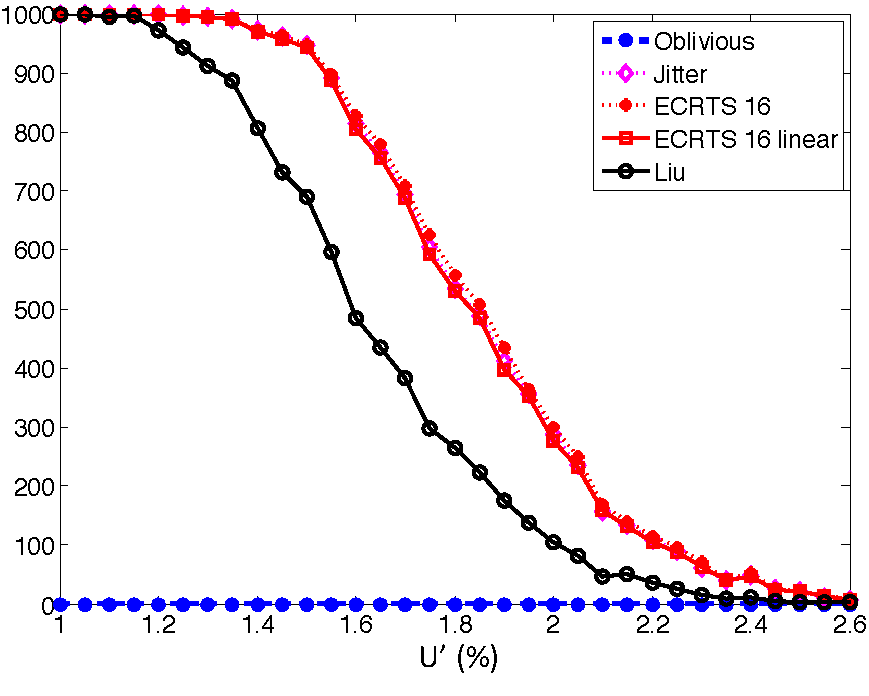
\includegraphics[width=0.23\textwidth]{../figures/experiments/varyingU_smin=50_smax=90_n=8_T=100-10000_1000runs_croped.pdf}} 
  \caption{Number of schedulable task sets over $1000$ randomly generated task sets.}
  \label{fig:exp}
\end{figure*}

Moreover, using the simple algebra property that for any two vectors $\vec{a}$ and $\vec{b}$ of size $(k-1)$ there is $\sum_{i=1}^{k-1} a_i \sum_{j=i}^{k-1} b_j = \sum_{j=1}^{k-1} b_j \sum_{i=1}^{j} a_i$, we get that $\sum_{i=1}^{k-1} U_i\sum_{\ell=i}^{k-1}x_\ell S_\ell = \sum_{i=1}^{k-1} x_i S_i \sum_{\ell=1}^{i}U_\ell $. Hence, injecting this last expression in Eq.~\eqref{eq:linear_step1}, it holds that
{\footnotesize
\begin{align*}
& C_k + S_k + \sum_{i=1}^{k-1}\ceiling{\frac{t+\sum_{\ell=i}^{k-1}x_\ell S_\ell+(1-x_i)(R_i-C_i)}{T_i}} C_i\\
\leq & C_k + S_k + \sum_{i=1}^{k-1}  \left(U_i\cdot t + C_i + U_i (1-x_i)(R_i-C_i) + x_i S_i\sum_{\ell=1}^{i}U_\ell \right)
\end{align*}}

It results that the minimum positive value for $t$ such that
{\footnotesize\begin{align}
\label{eq:linear-approximation-upper-bound}
C_k + S_k + \sum_{i=1}^{k-1}  \left(U_i t + C_i + U_i (1-x_i)(R_i-C_i) + x_i S_i\sum_{\ell=1}^{i}U_\ell \right) \leq t
\end{align}}
is an upper bound on the worst-case response time $R_k$ of $\tau_k$.

Observing Eq.~(\ref{eq:linear-approximation-upper-bound}), the
contribution of $x_i$ can be individually determined as $U_i(R_i-C_i)$
when $x_i$ is $0$ or $S_i(\sum_{\ell=1}^{i}U_\ell)$ when $x_i$ is
$1$. Therefore, whether $x_i$ should be set to $0$ or $1$ can be 
decided by individually comparing the two constants
$U_i(R_i-C_i)$ and $S_i(\sum_{\ell=1}^{i}U_\ell)$. Eq.~\eqref{eq:linear-approximation-upper-bound} is therefore minimized when $x_i=1$ if $U_i(R_i-C_i) > S_i(\sum_{\ell=1}^{i}U_\ell)$ and when $x_i = 0$ otherwise. We denote the resulting vector by $\vec{x}^{\mathit{lin}}$, where, for
each higher-priority task $\tau_i$,
\begin{equation}
\label{eq:x-linear}
x_i^{\mathit{lin}} =
\begin{cases}
1 & \text{if~} U_i(R_i-C_i) > S_i(\sum_{\ell=1}^{i}U_\ell) \\
0 & \text{otherwise}
\end{cases}
\end{equation}

The following properties directly follow.
\begin{Property}
For any $t > 0$, the vector assignment $\vec{x}^{\mathit{lin}}$ minimizes
  the solution to Eq.~\eqref{eq:linear-approximation-upper-bound} among all $2^{k-1}$ possible vector assignments.
\end{Property}



\begin{theorem}
\label{theorem:linear-time-test}
Let $rbf_k(t, \vec{x}^{\mathit{lin}})$ be the left hand side of Eq.~\eqref{eq:linear-approximation-upper-bound}. Task $\tau_k$ is schedulable
  under fixed-priority if
  \begin{equation}
    \label{eq:linear-time-test}
    rbf_k(D_k, \vec{x}^{\mathit{lin}}) \leq D_k.
  \end{equation}
\end{theorem}
\begin{proof}
  It directly follows from Corollary~\ref{corollary:general-framework}
  and the fact that, by construction,
  Eq.~\eqref{eq:linear-approximation-upper-bound} upper bounds
  Eq.~\eqref{eq:TDA-suspension-tighter0}. Note that $rbf_k(t,
  \vec{x}^{\mathit{lin}})$ can be expressed as $A+\sum_{i=1}^{k-1} U_i
  t$ with a constant $A > 0$ (independent from $t$). Therefore, if the
  condition in Eq.~\eqref{eq:linear-approximation-upper-bound} holds
  for a certain $0 < t < D_k$ with $A+\sum_{i=1}^{k-1} U_i t \leq t$, then
  the inequality $A+\sum_{i=1}^{k-1} U_i D_k \leq D_k$ also holds.
\end{proof}

\begin{Property}
The time complexity of both deriving $\vec{x}^{\mathit{lin}}$ and testing Eq.~(\ref{eq:linear-approximation-upper-bound}) is $O(k)$.
\end{Property}


% \begin{Corollary}
%   \label{corollary:linear-time-overall-test}
%   Considering task $\tau_k$ from $\tau_1, \tau_2, \ldots, \tau_n$, the
%   time complexity to test the schedulability of all these $n$ tasks is
%   $O(n)$ by using the test in
%   Theorem~\ref{theorem:linear-time-test}. Therefore, the amortized
%   time complexity to test task $\tau_k$ by using the test in
%   Theorem~\ref{theorem:linear-time-test} is constant.
% \end{Corollary}
% \begin{proof}
  
% \end{proof}




%%% Local Variables:
%%% mode: latex
%%% TeX-master: "master.tex"
%%% End:
